\chapter{Trabalhos Relacionados}
\label{cap:trabalhos-relacionados}

Neste capítulo, são apresentados os trabalhos relacionados na área de otimização de malhas com ruídos, mostrando as vantagens e desvantagens de cada técnica apresentada. Eles podem ser divididas basicamente em duas categorias: técnicas \textit{isotrópicas} e \textit{anisotrópicas}. Métodos isotrópicos são mais simples e só consideram informações intrínsecas ao modelo, enquanto métodos anisotrópicos, dentre os quais a técnica proposta se enquadra, usam outras informações, não inerentes diretamente ao modelo, para decidir como a filtragem deve ocorrer.

\section{Métodos isotrópicos}
O mais simples, e de melhor custo-benefício, método isotrópico é a suavização \textit{Laplaciana} (Figura \ref{fig:laplacian}), que move, iterativamente, todos os vértices do modelo em direção ao centro dos seus vizinhos, definindo, para cada vértice, a seguinte equação:
\begin{equation} \label{eq:laplacian}
    x_i = \frac{1}{N} \sum^{N}_{j=1} x_j,
\end{equation}
onde $N$ representa a quantidade de vértices adjacentes ao vértice de índice $i$, $x_j$ é a posição do vértice de índice $j$ adjacente ao vértice de índice $i$, e $x_i$ é a nova posição do vértice de índice $i$.

\begin{figure}[!h]
\captionsetup{width=\linewidth}
\centering
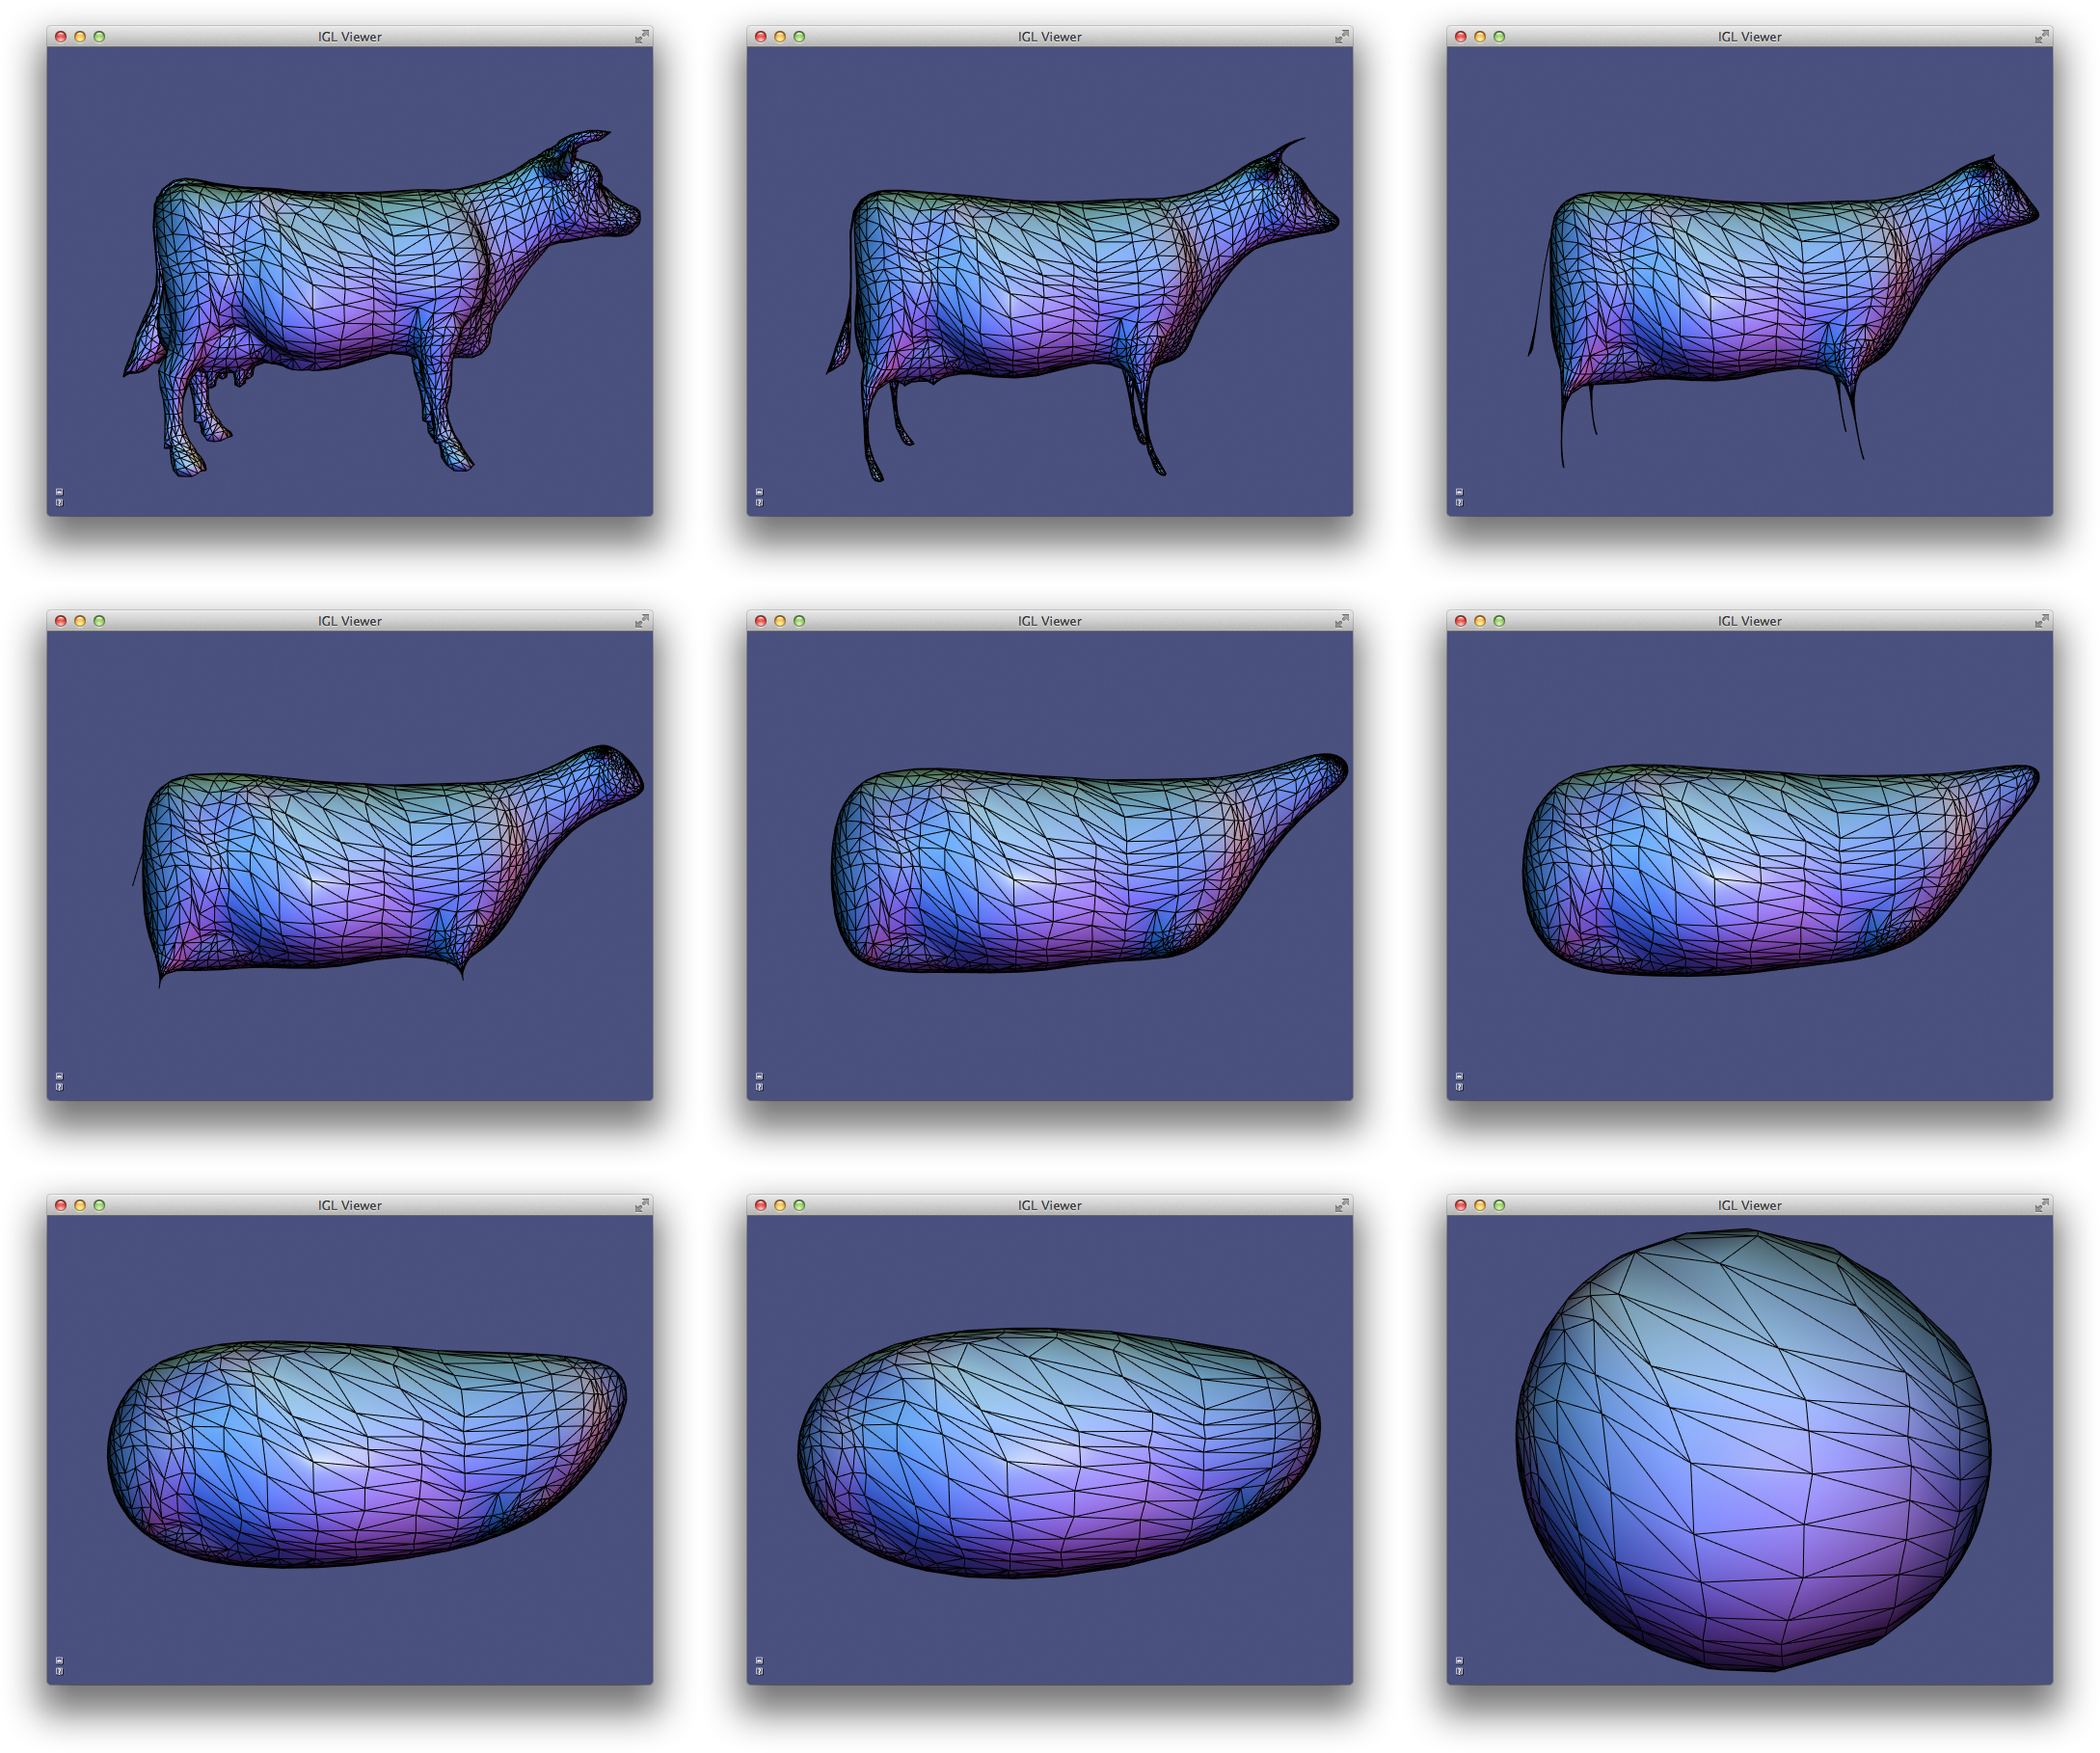
\includegraphics[scale=0.12]{figuras/laplacian.jpg}
\caption{Laplaciano aplicado ao modelo \textit{cow}. Redução de volume e perda de características podem ser notadas ao longo da aplicação do operador.}
\Fonte{http://libigl.github.io/}
\label{fig:laplacian}
\end{figure}

Apesar desta técnica ser muito rápida e simples, ela pode causar redução ou ampliação de volume e perda de características da malha, caso aplicada seguidas vezes, tornando-a não recomendável em um problema real.


Algumas melhorias foram apresentadas em \cite{vollmer1999improved} tentando resolver o problema da redução do volume ao aplicar uma operação de mover o vértice à sua posição original, depois de cada iteração. O vértice modificado $\mathbf{p}_i$ (produzido pelo \textit{Laplaciano}) é movido em direção ao vértice $\mathbf{q}_i$ e (ou) em direção ao vértice original $\mathbf{o}_i$ pela média das diferenças:
\begin{equation} \label{eq:drag-back}
    \mathbf{d}_i = -(\beta \mathbf{b}_i + \frac{1 - \beta}{|Adj(i)|} \sum_{j \in Adj(i)}{\mathbf{b}_j}),
\end{equation}
onde $\beta \in [0,1]$ é um escalar que define a influência do vértice central e seus vizinhos, $Adj(i)$ é o conjunto de vértices na vizinhança de $\mathbf{q}_i$ e $\mathbf{b}_i = \mathbf{p}_i - (\alpha \mathbf{o}_i + (1 - \alpha)\mathbf{q}_i)$, onde $\alpha \in [0,1]$ define a influência do vértice anterior $\mathbf{q}_i$ e do vértice original $\mathbf{o}_i$. A Figura \ref{fig:drag-back} ilustra a Equação \ref{eq:drag-back}.

\begin{figure}[!h]
\captionsetup{width=\linewidth}
\centering
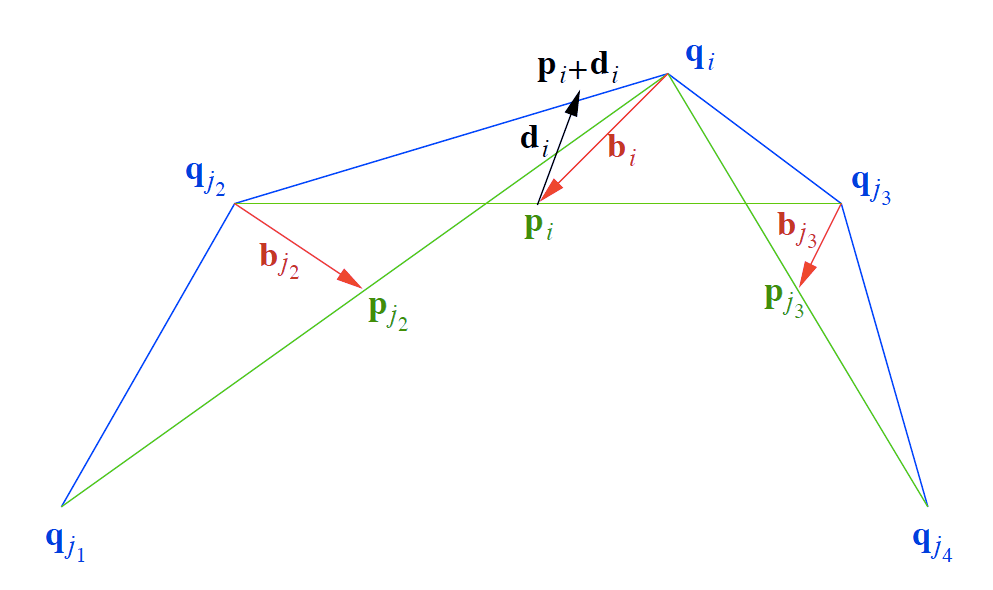
\includegraphics[scale=0.2]{figuras/drag-back-op.png}
\caption{Definição de $\mathbf{d}_i$ para mover os vértices produzidos pelo \textit{Laplaciano}. O vértice $\mathbf{o}_i$ não representado na figura, é o vértice na sua posição original antes de todas as iterações do Laplaciano.}
\Fonte{\cite{vollmer1999improved}}
\label{fig:drag-back}
\end{figure}

Esta técnica simples consegue resolver o problema da redução do volume encontrada no algoritmo de \textit{Laplace} (Figura \ref{fig:vollmerExample}) e possui algumas vantagens:
\begin{itemize}
    \item pode produzir malhas com mesmo grau de suavização do algoritmo de \textit{Laplace};
    \item preserva forma e volume da malha;
    \item rápida e de fácil implementação.
\end{itemize}

Porém, só apresenta bons resultados para modelos mais simples. Por ser uma técnica antiga, modelos mais complexos, como encontramos atualmente, não são contemplados.

\begin{figure}[!h]
\captionsetup{width=\linewidth}
\centering
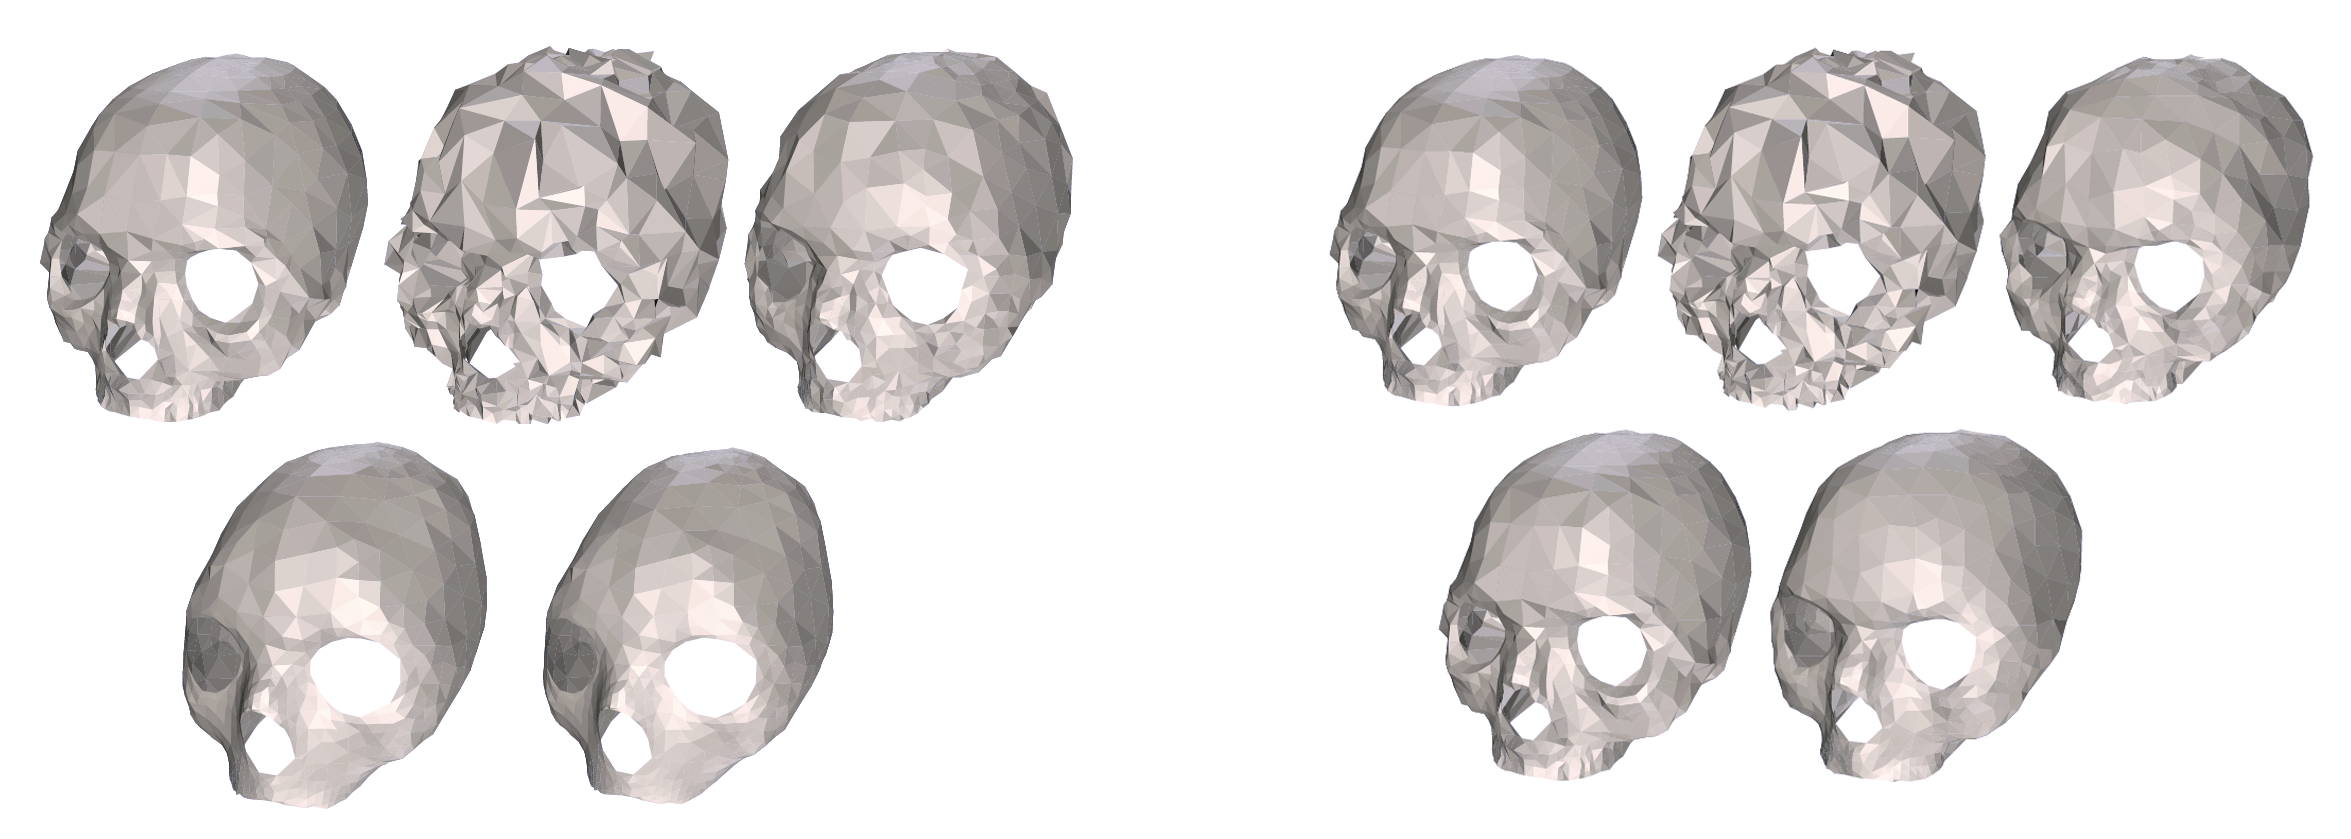
\includegraphics[width=\linewidth]{figuras/volmmerExample.png}
\caption{Esquerda: malha original, malha com ruído, 3 iterações de Laplace. Direita: malha original, malha com ruído, 3 iterações da técnica apresentada em \cite{vollmer1999improved}.}
\Fonte{\cite{vollmer1999improved}}
\label{fig:vollmerExample}
\end{figure}

Em \cite{liu2007non} um operador de otimização global é apresentado para malhas arbitrárias. Este operador global é composto de dois termos principais: operador Laplaciano global e condições de restrição para manter a fidelidade da malha. 

O operador Laplaciano, também conhecido como cordenadas diferenciais, pode ser aproximado em cada vértice pelo operador \textit{umbrella} (Figura \ref{fig:umbrella}):
\begin{equation}
    L(\mathbf{v}_i) = \sum_{j\in i^*}{w_{ij}(\mathbf{v}_j - \mathbf{v}_i}),
\end{equation}
onde $i^*$ é o conjunto de índices dos vértices vizinhos de $\mathbf{v}_i$, e $w_{ij}$ é o peso da aresta $(i,j)$ correspondendo ao vértice $\mathbf{v}_i$ com $\sum_{j\in i^*}{w_{ij} = 1}.$

\begin{figure}[!h]
\captionsetup{width=\linewidth}
\centering
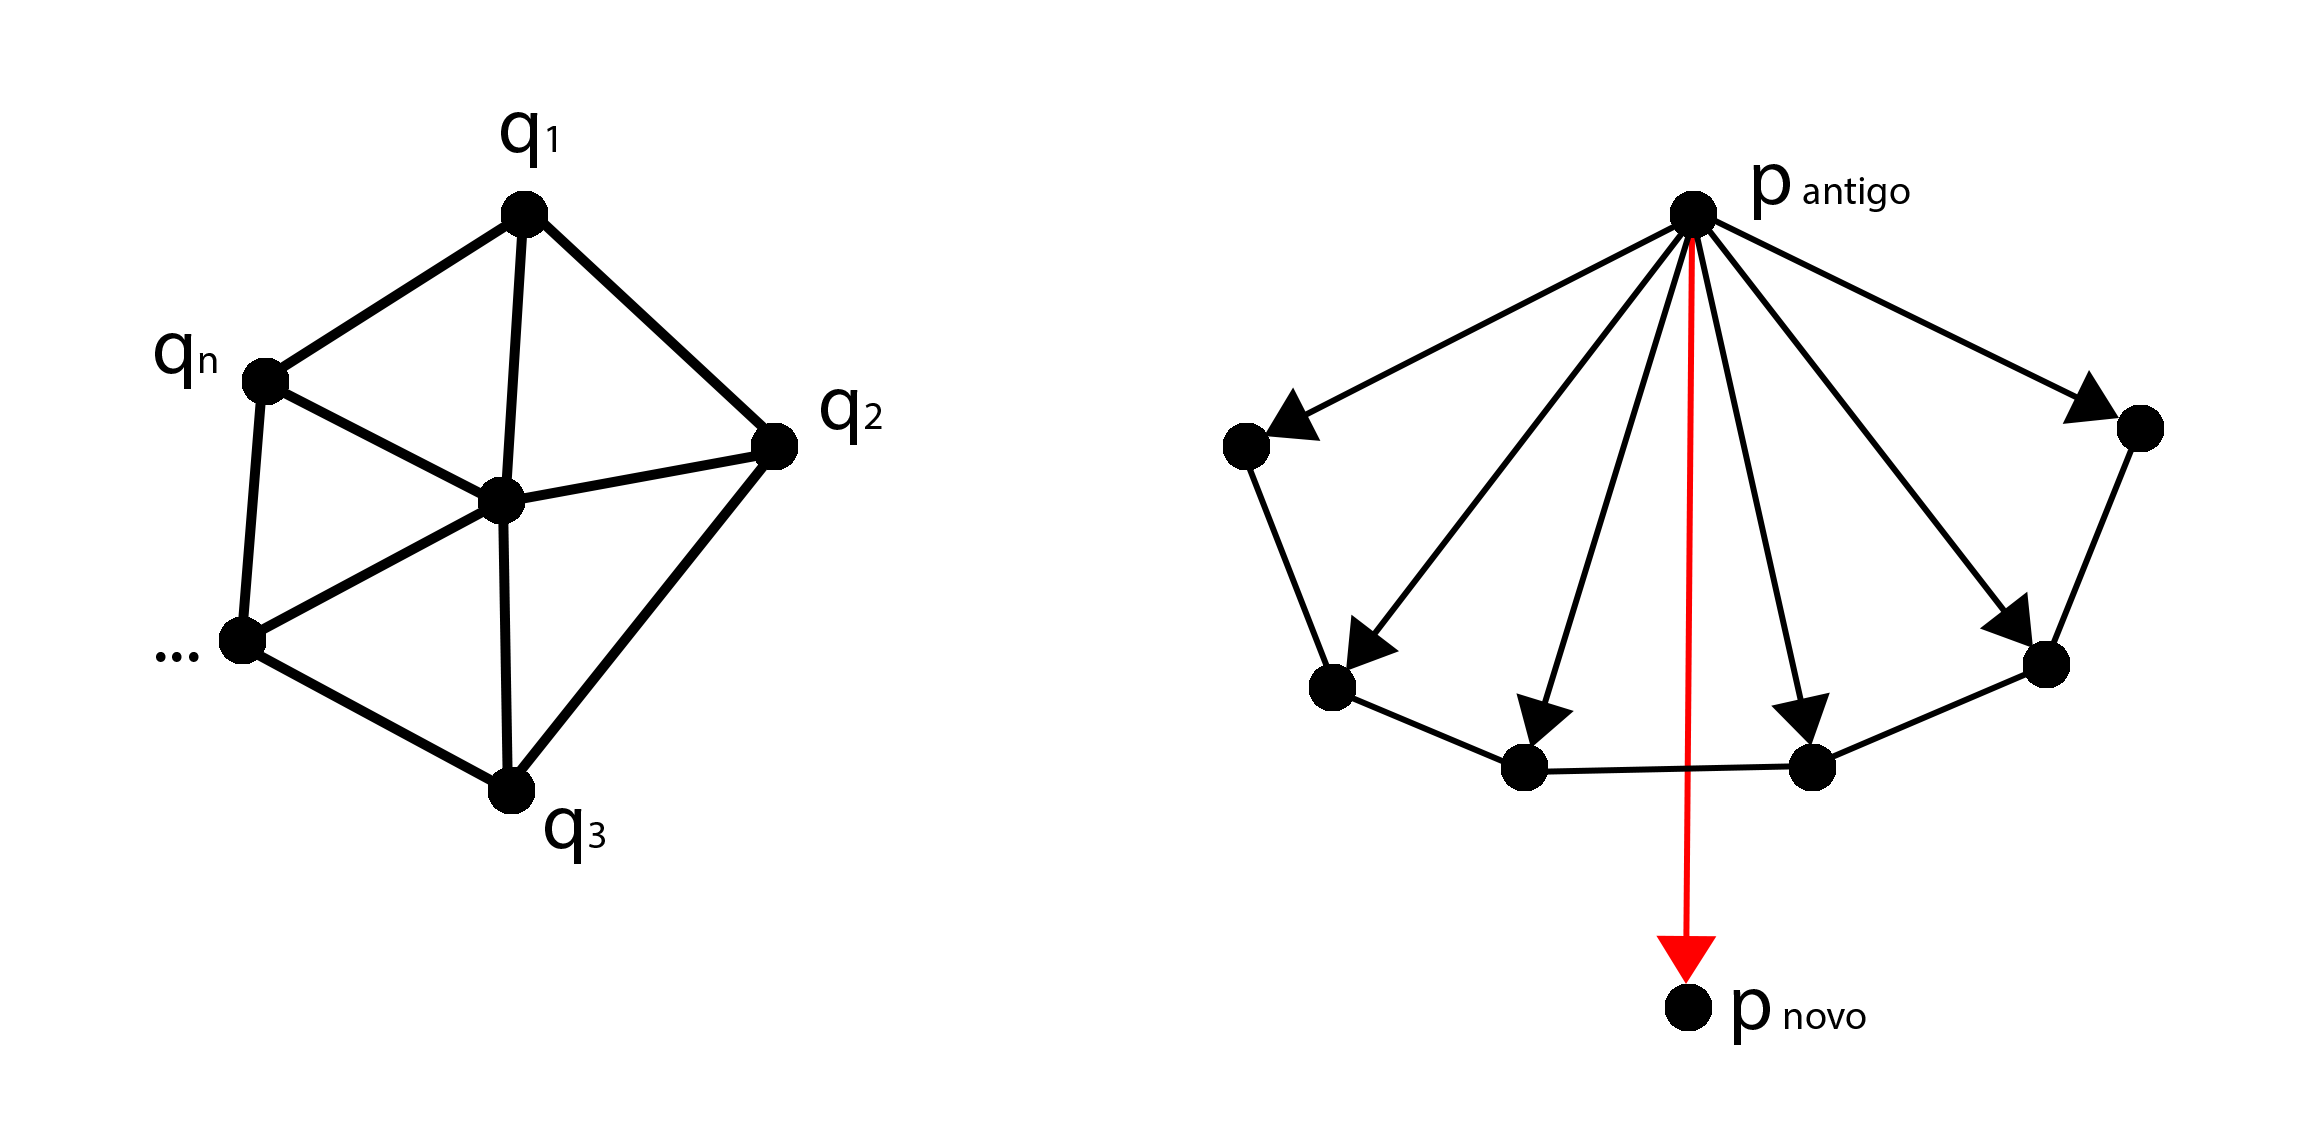
\includegraphics[scale=0.30]{figuras/umbrella_operator.png}
\caption{Definição do operador \textit{umbrella}. O ponto $p$ será movido pela média ponderada dos seus vizinhos $q_1$,.., $q_n$.}
\label{fig:umbrella}
\end{figure}

Foi observado que o vértice $\mathbf{v}_i$ permanece na média ponderada dos seus vizinhos imediatos (\textit{1-ring}) se a seguinte equação for satisfeita:
\begin{equation}
    \mathbf{v}_i - \sum_{j\in i^*}{w_{ij}\mathbf{v}_j} = 0,
\end{equation}
portanto, isto também é considerado na criação do Laplaciano global. As condições de otimização global para todos os vértices é definida da seguinte forma:
\begin{equation}
    \mathbf{L}\mathbf{X} = 0,
\end{equation}
onde $\mathbf{L}$ é uma matriz $n$ x $n$ com elementos derivados de $w_{ij}$:
\begin{equation}
L_{ij}=\left\{
\begin{array}{c l}	
     1, & i=j,\\
     -w_{ij} & (i,j) \in E, \\
     0 & c.c,
\end{array}\right.
\end{equation}
onde $X$ é o vetor coluna dos vértices correspondentes e $E$ é o conjunto de arestas da malha. Formando, dessa forma, toda a restrição de otimização do Laplaciano global.

Restrições de vértices (Figura \ref{fig:restricao_vertices}) e restrições de baricentro das faces também são aplicadas para manter características da malha. Esses vértices são detectados automaticamente ou com a ajuda do usuário.

\begin{figure}[!h]
\captionsetup{width=\linewidth}
\centering
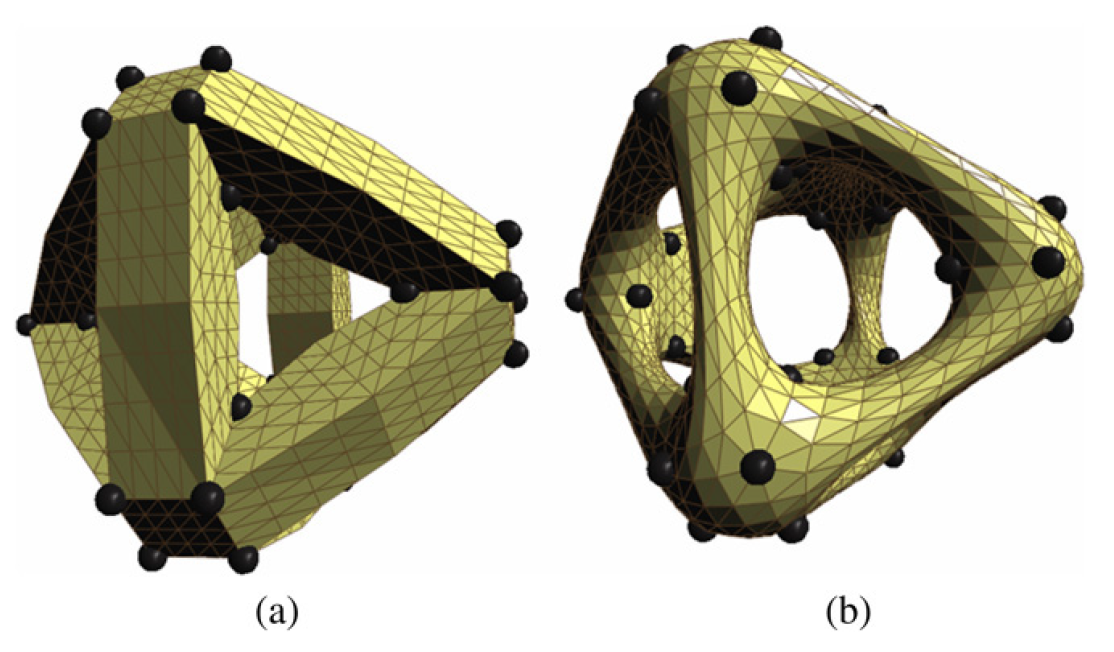
\includegraphics[scale=0.25]{figuras/restricao_vertices.png}
\caption{Otimização Laplaciana global com restrição de vértices. Os vértices da restrição estão na cor preta em destaque: (a) malha original; (b) malha otimizada.}
\Fonte{\cite{liu2007non}}
\label{fig:restricao_vertices}
\end{figure}

Apesar de resultados relevantes (Figura \ref{fig:dragon_laplaciano_global}) e da grande contribuição dos métodos isotrópicos para a área de otimização de malhas, métodos baseados no Laplaciano geralmente não conseguem preservar características e volume da malha, enquanto remove os ruídos existentes.

\clearpage

\begin{figure}[!h]
\captionsetup{width=\linewidth}
\centering
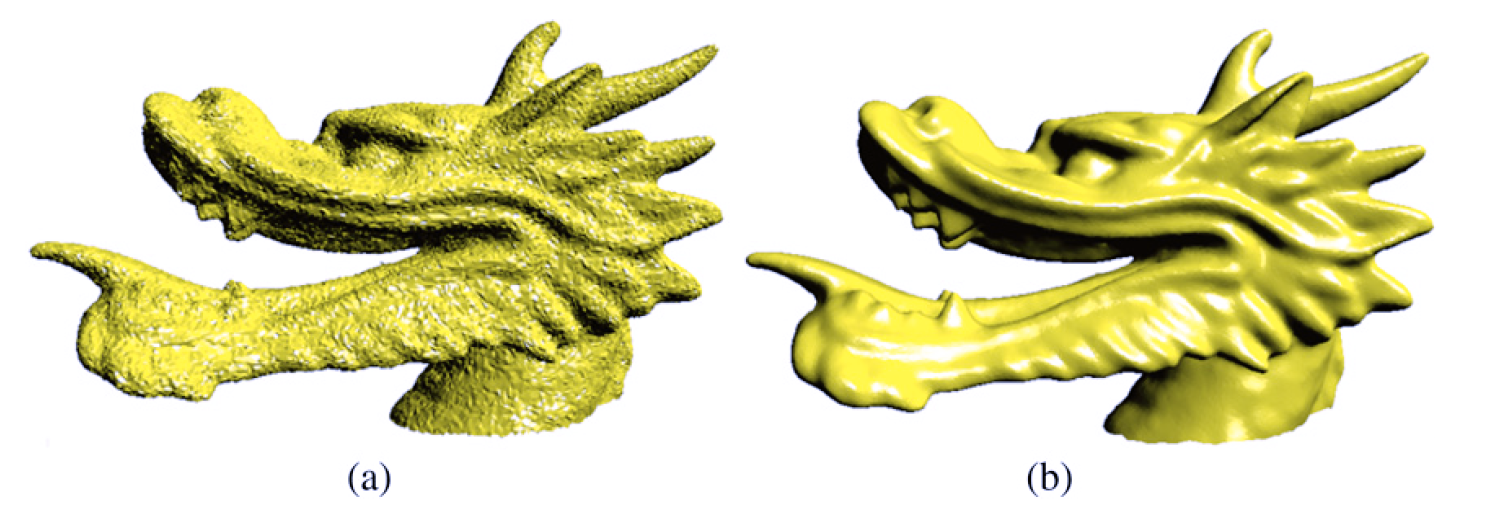
\includegraphics[scale=0.28]{figuras/dragon_laplaciano_global.png}
\caption{Resultado do uso da técnica de \cite{liu2007non}, no modelo \textit{dragon}, para remoção de ruídos: (a) o modelo \textit{dragon} com ruído; (b) o modelo \textit{dragon} otimizado com restrições de vértices e baricentro de faces.}
\Fonte{\cite{liu2007non}}
\label{fig:dragon_laplaciano_global}
\end{figure}


\section{Métodos anisotrópicos}

Neste mesmo contexto, uma variedade de métodos anisotrópicos foram criados no intuito de uma melhor preservação das características geométricas do modelo. Alguns deles se inspiraram nos conceitos propostos em processamento de imagens, como a filtragem bilateral \cite{tomasi1998bilateral}, que é, essencialmente, um filtro não-linear, para suavização de imagens, que preserva características importantes, tais como as arestas. Esta técnica substitui o valor de intensidade de um pixel pela média ponderada dos valores de intensidade dos pixels próximos. Desta forma, um pixel só é influenciado por pixels próximos com intensidade similares. A filtragem bilateral para uma imagem $I(\mathbf{u})$, em uma coordenada $\mathbf{u} = (x,y)$ é definida em \cite{tomasi1998bilateral} como:
\begin{equation}\label{eq:filtro_bilateral} 
    \hat{\mathrm{I}}(\mathbf{u}) = \frac{\sum_{p \in N(\mathbf{u})}{W_c(\|\mathbf{p}-\mathbf{u}\|)W_s(|I(\mathbf{u})-I(\mathbf{p})|)I(\mathbf{p})}}{ \sum_{p \in N(\mathbf{u})}{W_c(\|\mathbf{p}-\mathbf{u}\|)W_s(|I(\mathbf{u})-I(\mathbf{p})|)} },
\end{equation}
onde $N(\mathbf{u})$ é a vizinhança de pixels de $\mathbf{u}$, $W_c(x) = e^{-x^2/2\sigma_c^2}$, com parâmetro $\sigma_c$, representa o kernel Gaussiano de proximidade e $W_s(x) = e^{-x^2/2\sigma_s^2}$, com parâmetro $\sigma_s$, representa o kernel de intensidade.

O sucesso dessa abordagem em processamento de imagens levou à sua adaptação na área de processamento de geometria, em técnicas de remoção de ruído e suavização de malhas \cite{fleishman2003bilateral, jones2003non, zheng2011bilateral, solomon2014general}.

Em \cite{fleishman2003bilateral}, os vértices são filtrados na direção da normal usando-se os seus vizinhos locais. A técnica parte do pressuposto de que todo vértice $v$ na malha com ruído está a uma distância $d_v$ para a malha \textit{ground-truth}, que é a malha completamente sem ruído utilizada para comparação do resultado da otimização da malha com ruído. Portanto essa distância é estimada aplicando o filtro iterativamente, atualizando $v$ da seguinte forma:
\begin{equation}
    v = v + d \cdot n,
\end{equation}
onde $n$ é o vetor normal associado a $v$, que irá direcionar o deslocamento de $v$. O filtro é aplicado a cada vértice, calculando o seu deslocamento e atualizando sua posição baseada na Equação \ref{eq:filtro_bilateral}.

Em \cite{jones2003non}, uma técnica de filtragem bilateral de malhas com ruídos, baseada em estimativas estatísticas robustas, é apresentada. O modelo se baseia na afirmação de que uma técnica de suavização, que preserva as características da malha, pode ser vista meramente como um problema de estimar uma superfície na presença de \textit{outliers}. A extensão de métodos estatísticos robustos para técnicas de filtragem de superfície não é algo trivial. Para a obtenção da suavidade de uma superfície, são definidos preditores locais de primeira ordem (Figura \ref{fig:predictions}). Com um estimador robusto, são achadas as novas posições de cada vértice como uma soma ponderada das predições na sua vizinhança espacial.


\begin{figure}[!h]
\captionsetup{width=\linewidth}
\centering
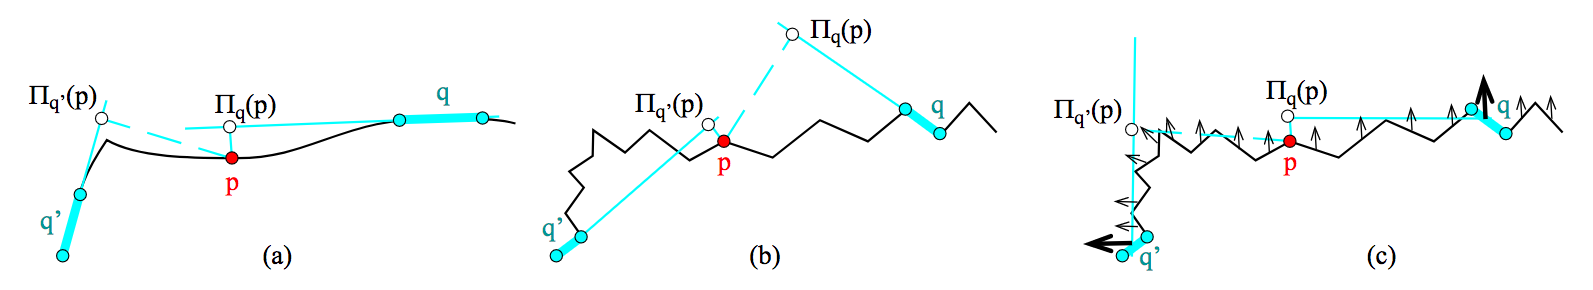
\includegraphics[scale=0.28]{figuras/predictions.png}
\caption{(a) A predição $\Pi_q(p)$ para um ponto $p$, baseado na superfície de $q$, é a projeção de $p$ no plano tangente formado pela superfície de $q$. Pontos em regiões de linhas características (arestas) resultam em predições mais distantes e, portanto, causando menos influência. (b) Normais com ruídos podem levar a más predições. (c) Normais melhoradas mitigam este problema, pois os planos tangentes são construídos baseados nelas. }
\Fonte{\cite{jones2003non}}
\label{fig:predictions}
\end{figure}

Apesar de apresentar bons resultados, e mostrar que a filtragem bilateral é robusta a \textit{outliers}, esse método depende, fortemente, da aproximação dos preditores locais, e estes são muito sensíveis a ruídos, mesmo com o passo de melhoria das normais. 

A eficácia da filtragem bilateral foi estendida pela filtragem bilateral conjunta (\textit{joint}) em \cite{eisemann2004flash}, \cite{petschnigg2004digital}. A ideia é que os pesos associados podem ser determinados usando as diferenças de intensidades de uma outra imagem, chamada \textbf{guia} (Figura \ref{fig:flash-noflash}). A filtragem bilateral conjunta atinge melhores resultados que a filtragem bilateral clássica, quando a imagem guia proporciona melhores informações do que a imagem de entrada a ser tratada. A filtragem bilateral conjunta foi usada com sucesso em processamento de imagens, conseguindo bons resultados. O verdadeiro desafio é a sua adaptação aos sinais geométricos, para que possa ser usado, também, em técnicas de otimização de malhas. Diferentemente dos sinais definidos nas imagens (e.g valor de intensidade em um pixel), que estão limitados a domínios simples e retangulares, os sinais geométricos (e.g posição de um vértice, normais, planos tangentes etc) são, geralmente, definidos em relação à superfície da malha, que possui topologia arbitrária e amostragem de elementos irregular. Esse guia geométrico tem que ser, comumente, construído computacionalmente.

\begin{figure}[!h]
\captionsetup{width=\linewidth}
\centering
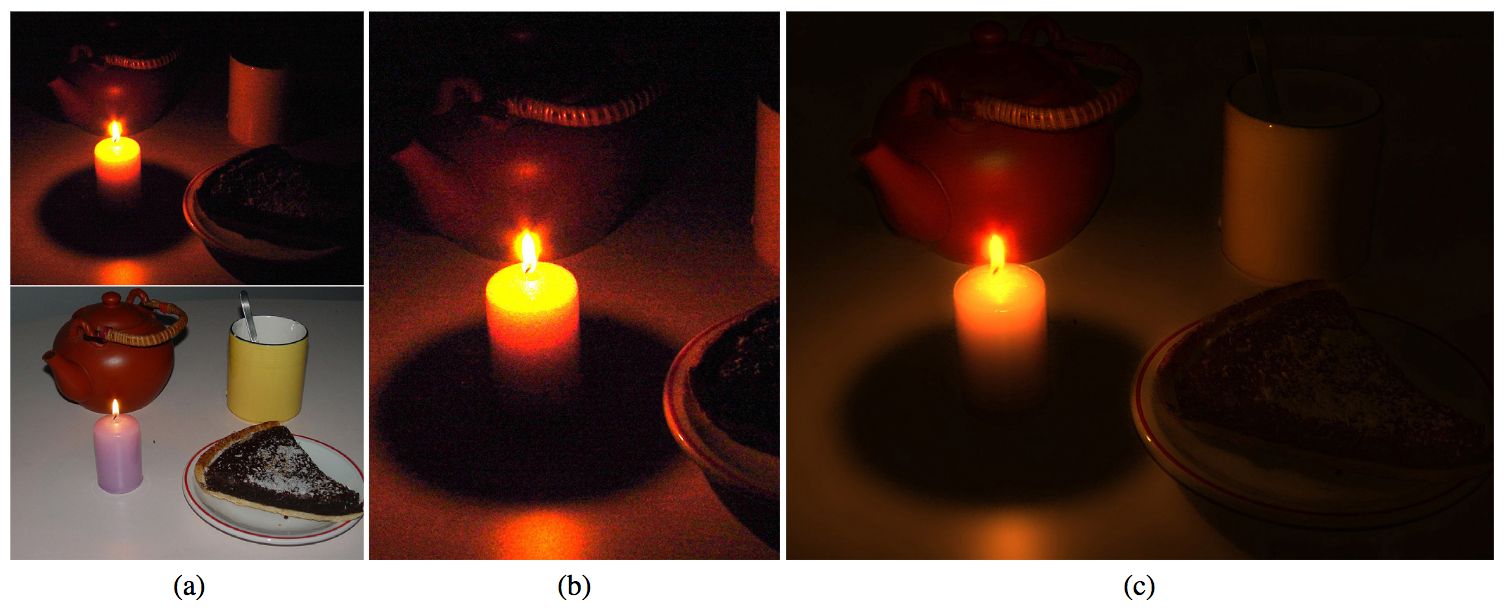
\includegraphics[scale=0.3]{figuras/flash-noflash.png}
\caption{(a) Cima: Fotografia tirada em um ambiente escuro, a imagem possui ruído e embaçamento. Baixo: Mesma fotografia com flash, provendo uma imagem com maiores detalhes, porém plana e possuindo sombras indesejadas na silhueta dos objetos. (b) Ampliação da imagem mostrando o ruído presente. (c) Técnica de \cite{eisemann2004flash} misturando as duas imagens (com flash e sem flash) para transferir a luz do ambiente à imagem principal.}
\Fonte{\cite{eisemann2004flash}}
\label{fig:flash-noflash}
\end{figure}

Em \cite{zheng2011bilateral} também é apresentada uma técnica baseada no filtro bilateral de \cite{tomasi1998bilateral} e o filtro bilateral conjunto de \cite{eisemann2004flash} e \cite{petschnigg2004digital}. São apresentados dois esquemas de remoção de ruídos. Além da abordagem de aplicar o filtro bilateral nas normais da malha com uma formulação iterativa e local (apenas considerando a intensidade das normais na vizinhança), é apresentado, também, uma formulação, não iterativa, global para remoção de ruídos em malhas. É mostrado que a formulação global é mais robusta para malhas com ruídos possuindo triangulações irregulares, enquanto que a formulação local recupera mais rapidamente, e mais efetivamente, malhas com uma maior quantidade e intensidade de ruídos (Figura \ref{fig:globalxlocal}).

\begin{figure}[!h]
\captionsetup{width=\linewidth}
\centering
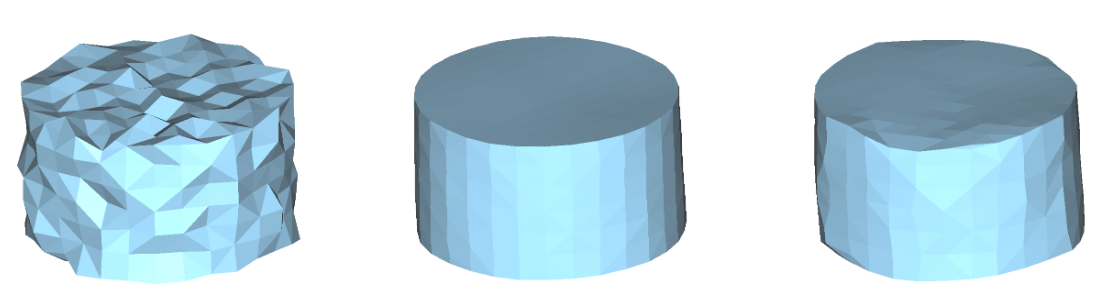
\includegraphics[scale=0.3]{figuras/globalxlocal.png}
\caption{Remoção de ruídos do modelo cilíndro (a esquerda). A formulação local (meio) recupera, mais eficientemente, as características geométricas do que a formulação global (direita) quando o nível de ruído é elevado.}
\Fonte{\cite{zheng2011bilateral}}
\label{fig:globalxlocal}
\end{figure}

Em \cite{solomon2014general}, uma generalização do filtro bilateral é apresentada. Um \textit{framework} que pode ser usado para suavizar sinais definidos em imagens, malhas e outros domínios. A construção da técnica é reduzida, exatamente, ao filtro bilateral para imagens em domínios retangulares. É mostrado também a aplicação do \textit{framework} a outros efeitos geométricos como o aprimoramento de características. A principal contribuição da técnica é a maior customização dos \textit{kernels} definidos no filtro bilateral (Figura \ref{fig:kernelframework}), fazendo com que seja possível aplicar a técnica de uma forma generalizada e em várias aplicações.

\begin{figure}[!h]
\captionsetup{width=\linewidth}
\centering
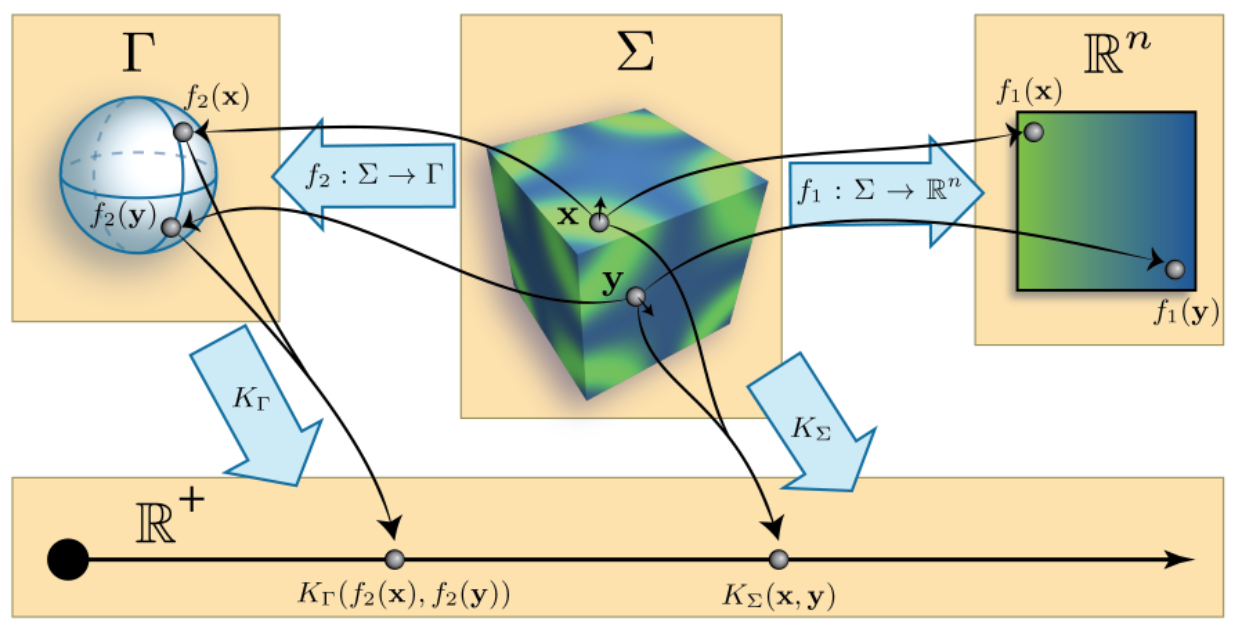
\includegraphics[scale=0.3]{figuras/kernelframework.png}
\caption{\textit{Kernels} $f_1$ e $f_2$ definidos em relação a uma esfera e a uma textura, respectivamente.}
\Fonte{\cite{solomon2014general}}
\label{fig:kernelframework}
\end{figure}

Em suma, \cite{fleishman2003bilateral} e \cite{jones2003non} usam a filtragem bilateral simples, aplicando o filtro diretamente nos vértices da malha, enquanto \cite{zheng2011bilateral} e \cite{solomon2014general} aplicam a filtragem bilateral conjunta nas normais das faces, seguido de uma atualização nas posições dos vértices baseada nas normais filtradas. A dificuldade encontrada nesse processo advém da natureza das normais encontradas em modelos com ruídos, que geralmente estão corrompidas pelo próprio ruído da malha, não sendo um bom guia para a filtragem bilateral conjunta, levando assim a resultados insatisfatórios.

Em \cite{zhang2015guided}, é mostrado como calcular um campo de normais guia mais confiável e robusto para a filtragem bilateral conjunta de malhas com ruídos. As novas normais guias serão computadas a partir da média das normais das faces vizinhas, e essas novas normais irão guiar a atualização dos vértices da malha (no trabalho proposto nessa dissertação, a mesma construção do campo de normais guia será utilizada, portanto mais detalhes sobre este processo serão descritos no Capítulo \ref{chap:tecnicaproposta}). A abordagem de usar a filtragem bilateral conjunta nas normais das faces e atualizar as posições dos vértices a partir dessas normais também foi adotada por muitos outros trabalhos \cite{sun2007fast, yagou2002mesh, chen2005sharpness, sun2008random}, diferindo entre eles na estratégia de filtragem das normais. Todos esses métodos anisotrópicos são focados principalmente em preservar características do modelo no processo de remoção de ruído, demonstrando pouca atenção na melhoria da qualidade da malha. Afim de otimizar uma malha com ruído enquanto melhora sua regularidade, \cite{wei2013feature} apresentam um método de dois passos que usa a filtragem bilateral conjunta juntamente com a suavização Laplaciana com restrições (Figura \ref{fig:filtroEregularidade}). 

\begin{figure}[!h]
\captionsetup{width=\linewidth}
\centering
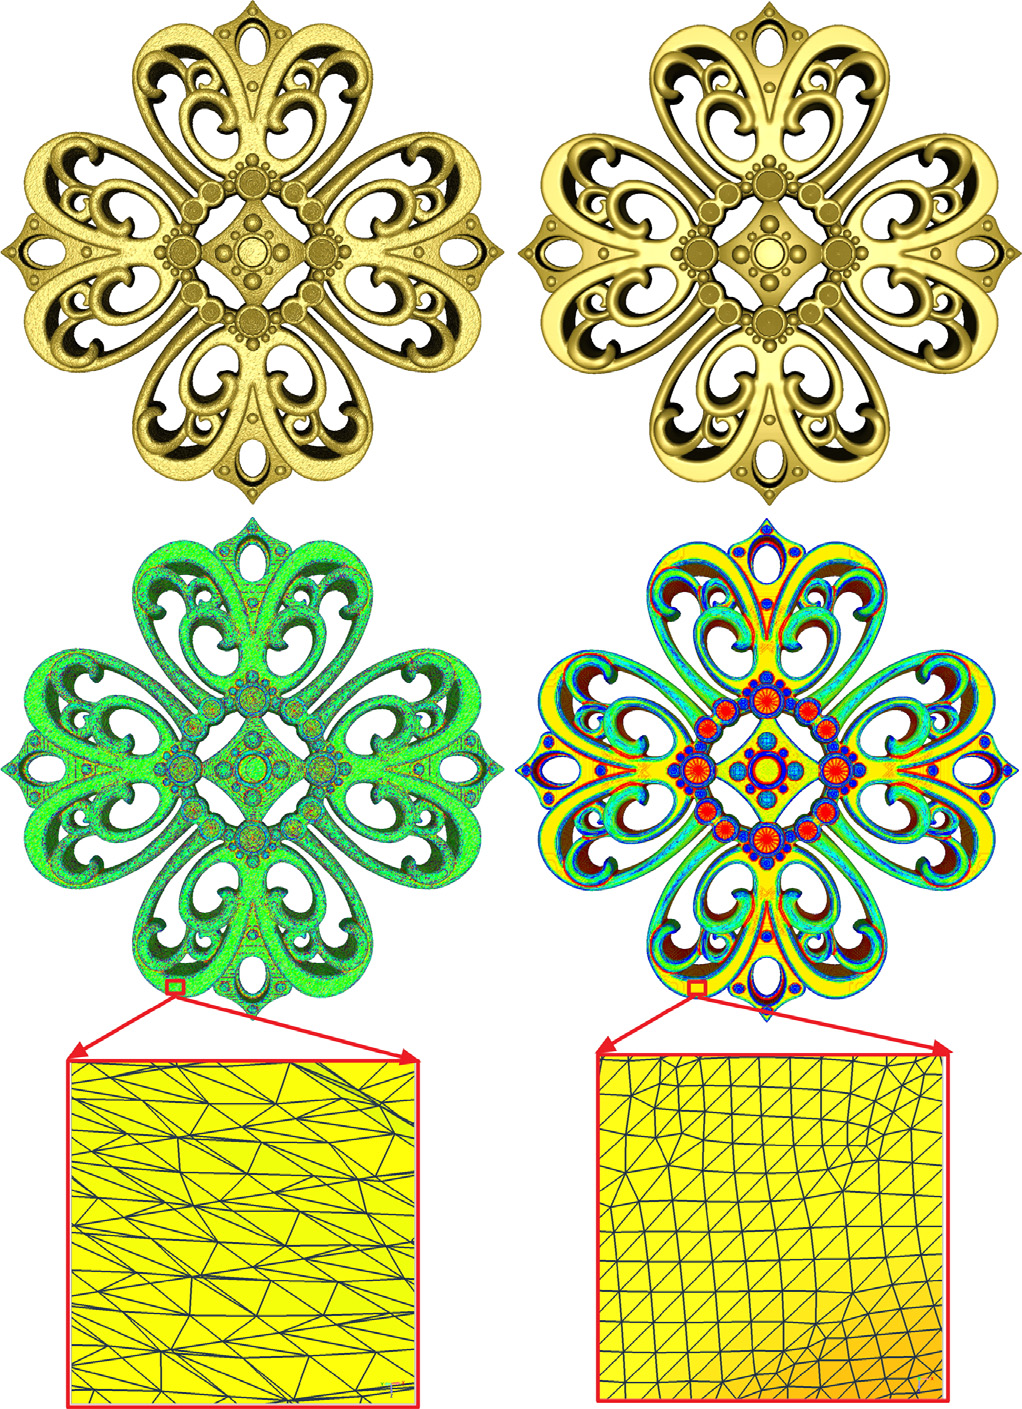
\includegraphics[scale=0.2]{figuras/filtroEregularidade.png}
\caption{Otimização do modelo \textit{Filgree} usando a técnica proposta em \cite{wei2013feature}. A primeira linha mostra a geometria do modelo com ruído (esquerda) e do modelo otimizado (direita). A linha do meio ilustra a visualização da curvatura média, e a linha de baixo mostra os fragmentos ampliados.}
\Fonte{\cite{wei2013feature}}
\label{fig:filtroEregularidade}
\end{figure}

\section{Considerações Finais}

As técnicas discutidas neste capítulo apresentam bons resultados na maioria dos casos, mas falham em otimizar malhas com grande presença de ruídos ou com amostragem de faces extremamente irregular (Figura \ref{fig:irregularSampling}). Não há garantia de que modelos gerados a partir de um \textit{scanner} 3D possuam uma malha com amostragem regular de faces. Desta forma, uma técnica de otimização de modelos com ruídos pode gerar resultados indesejados.

\begin{figure}[!h]
\captionsetup{width=\linewidth}
\centering
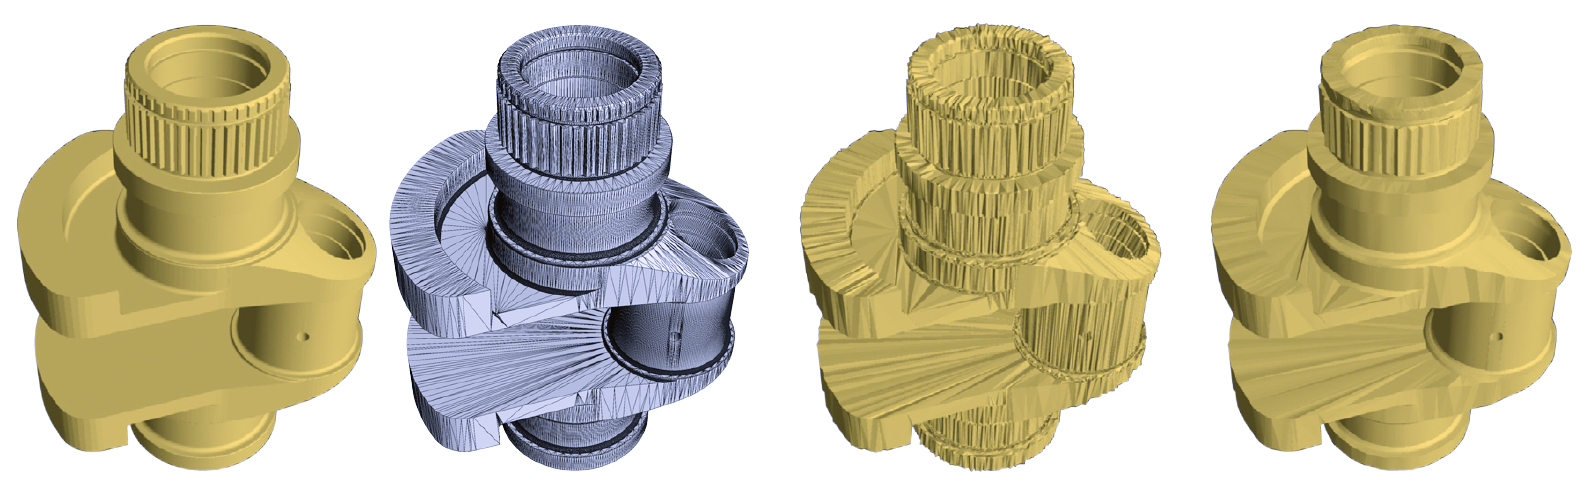
\includegraphics[width=\linewidth]{figuras/irregularSampling.png}
\caption{Da esquerda para a direita: Modelo sem ruído (\textit{ground-truth}), \textit{ground-truth} mostrando a malha associada ao modelo, modelo com ruído sintético, resultado da técnica de \cite{zhang2015guided}. }
\Fonte{\cite{zhang2015guided}}
\label{fig:irregularSampling}
\end{figure}













%\Gls{ambiguidade}
%\Gls{braile}
%\Gls{coerencia}
%\Gls{dialetos}
%\Gls{elipse}
%\Gls{locucao-adjetiva}
%\Gls{modificadores}
%\Gls{paronimos}
%\Gls{sintese}
%\Gls{borboleta}